

\chapter{Surface Imaging}

\section{Introduction}

The AFM used for imaging was the Bruker Nanoscope 2, which contains a sample mounted on a 1cm disc, atop the J scanner piezo. The head unit is then held down using springs, and a mirror used to align the laser onto the mounted cantilever.



\begin{figure}[h!!!!!!!]     %Insert a figure as soon as possible
        \begin{center}
          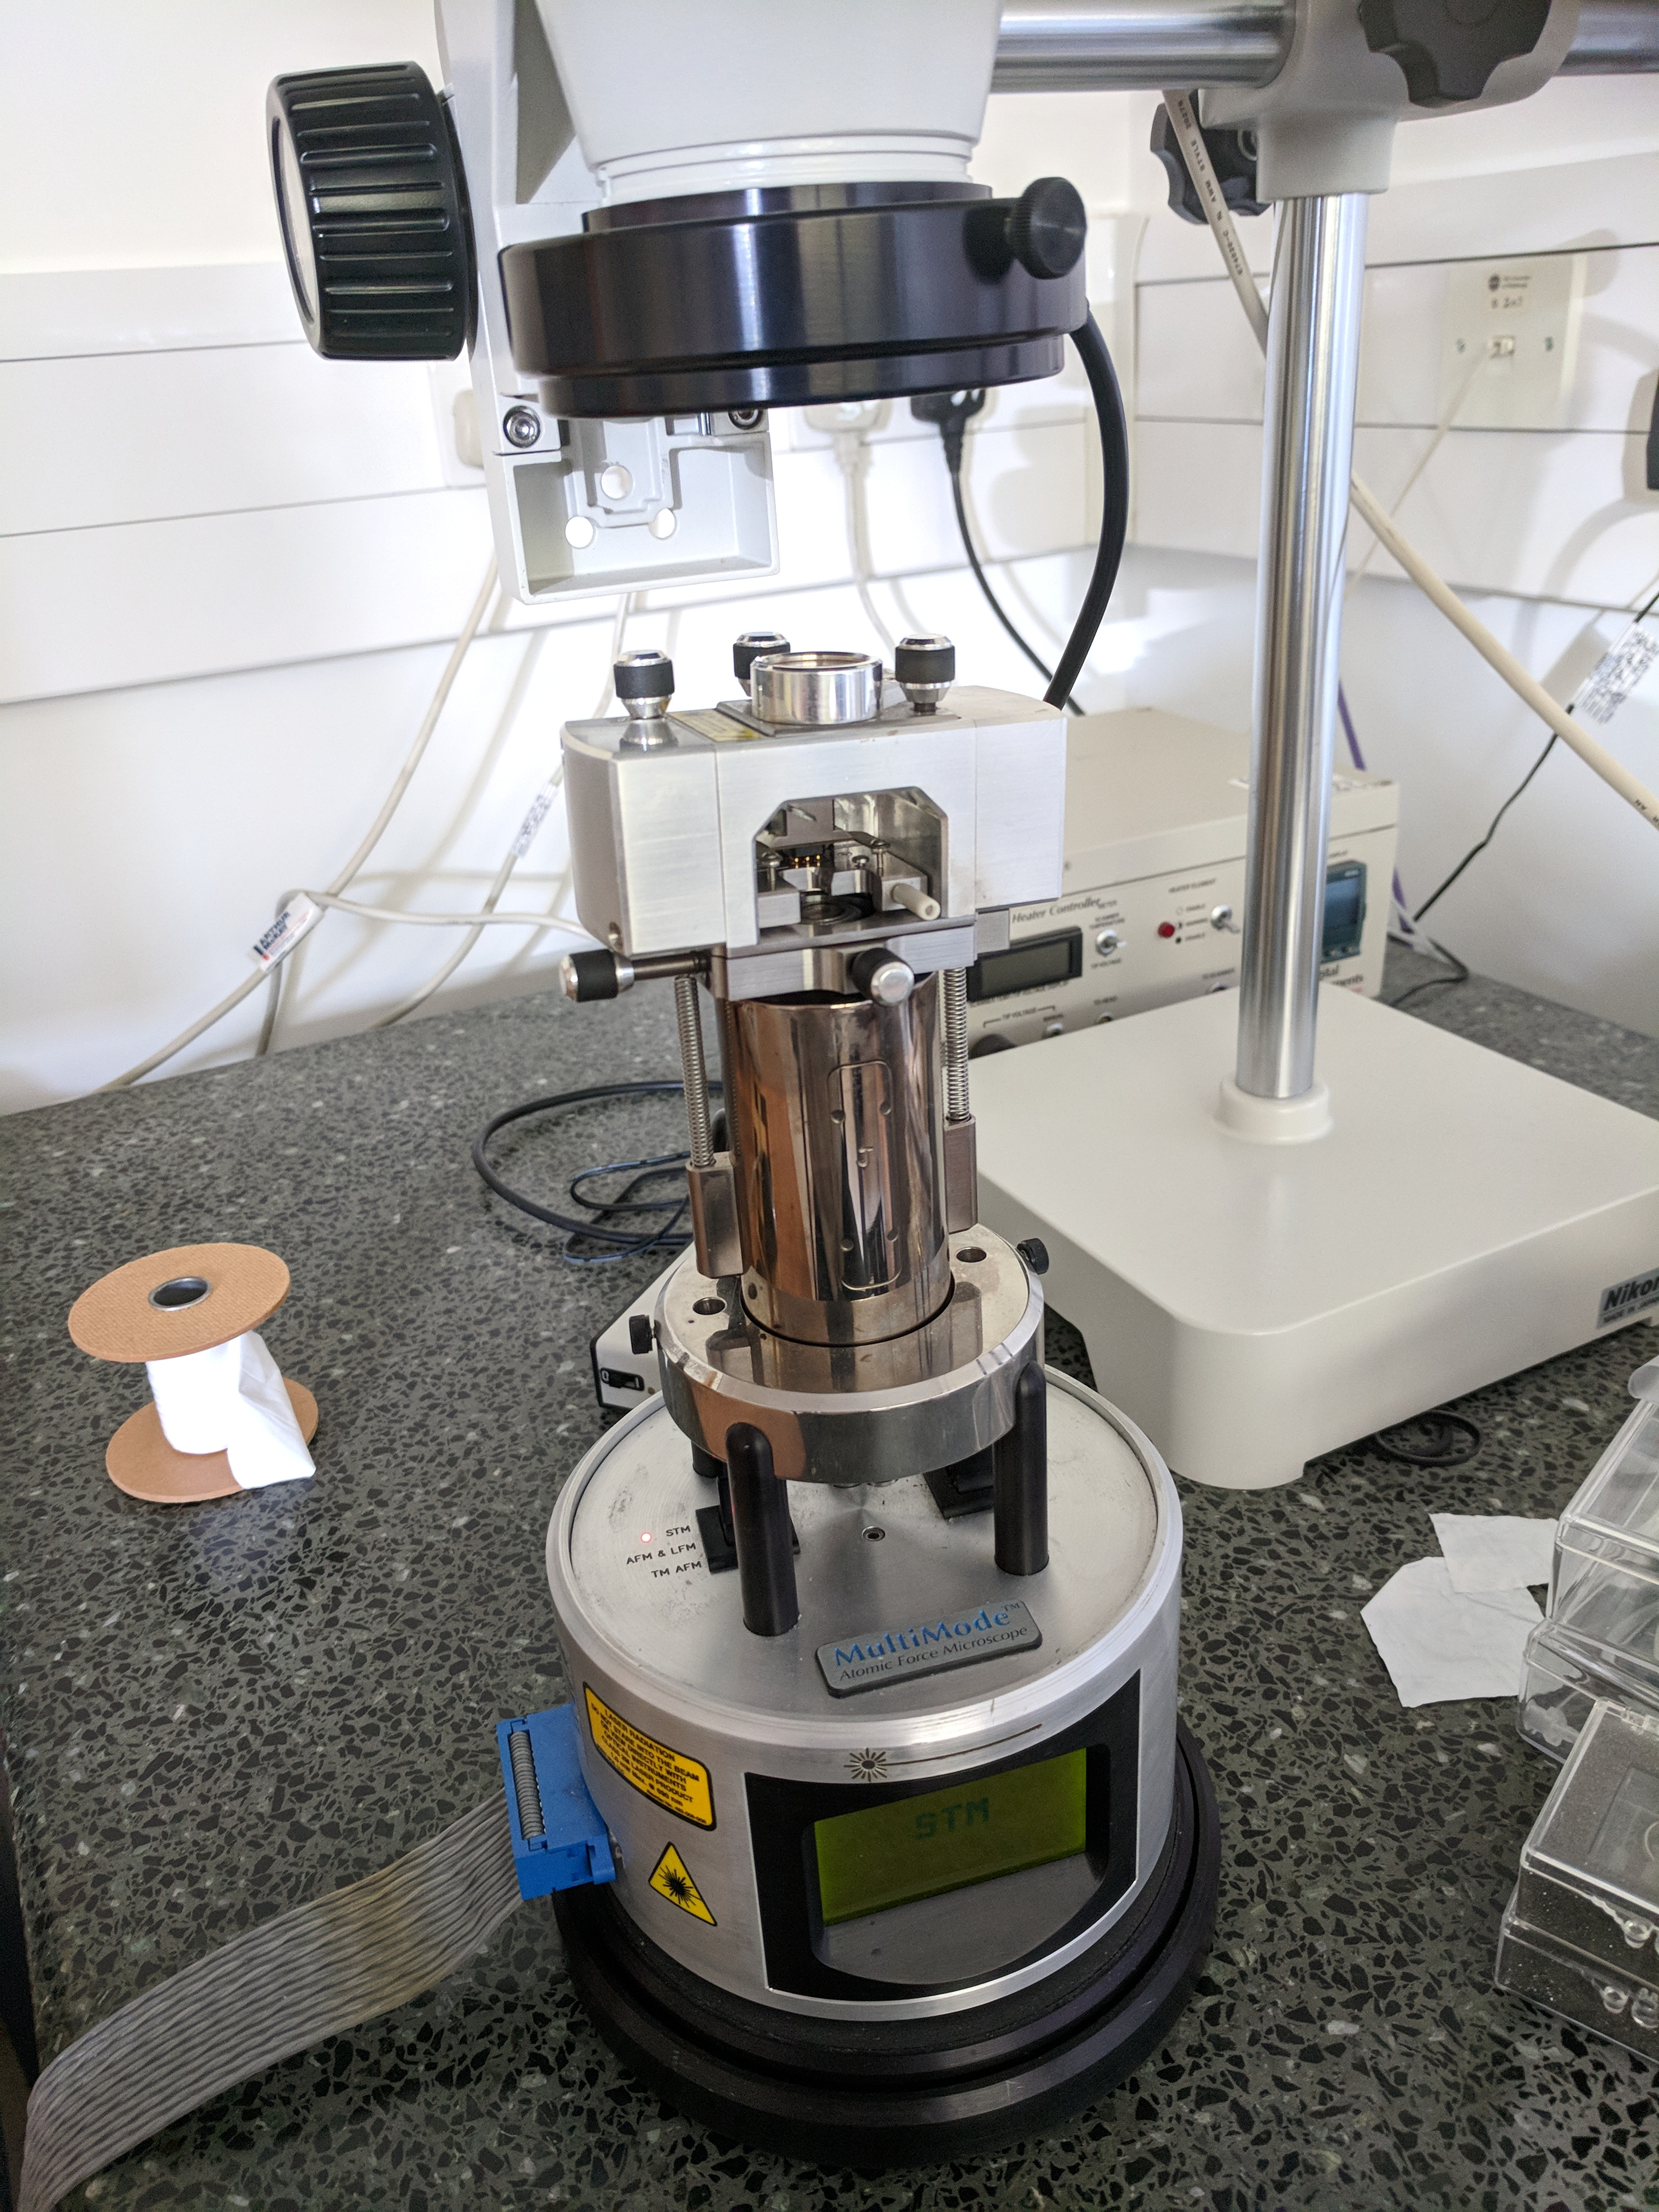
\includegraphics[width=110mm]{chapter2/ImageAFM.jpg}
\end{center}
\caption{Photograph of the operational setup for the Bruker Nanoscope 2, which was used for image measurements.}
\label{fig:ImageAFM}                 % Reference label to the figure.
\end{figure}

In order to characterise the borosilicate glass capillaries used an Atomic force microscopy (AFM) investigation was performed. This intended to investigate the uniformity of a borosilicate capillary across multiple capillaries by profiling the surface topology and roughness within the same length scale of the cantilver heads. This glass capiliary was then cross referenced against the petri dish in use, to ensure that the surface of the petri dish was representative of borosilicate glass. This surface was then referenced against scanning electron microscopy images of the tips, alongside inverted AFM imaging of the tip.

Initially the inside of a glass capillary was imaged.

\begin{figure}[h]     %Insert a figure as soon as possible
        \begin{center}
          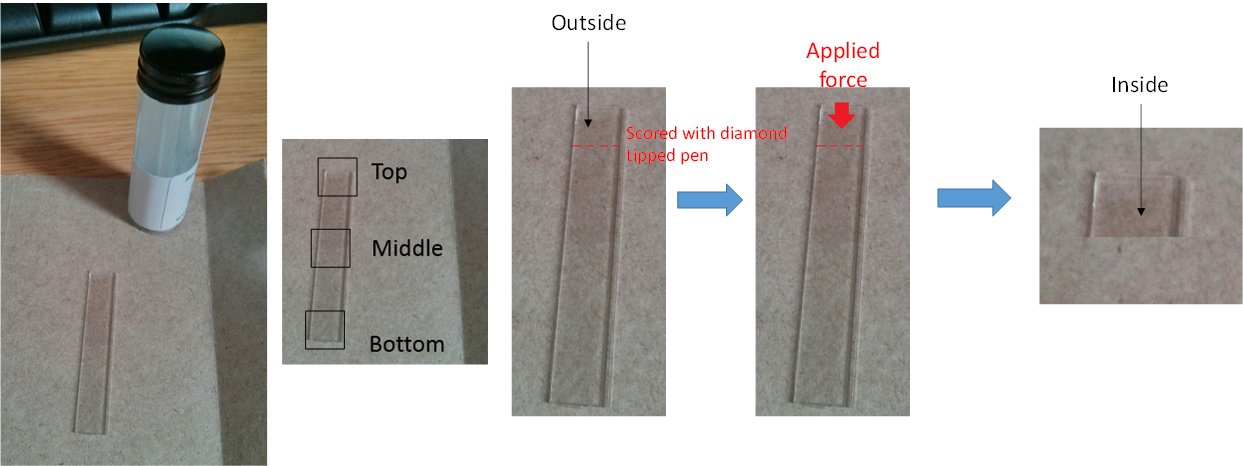
\includegraphics[width=120mm]{chapter3/Figure8.png}
\end{center}
\caption{A diagram demonstrating how the glass capillary was broken and how samples were extracted from the capillary.}
\label{fig:figure8}                 % Reference label to the figure.
\end{figure}   

The inside of the capillary was imaged by scoring the glass with a diamond tipped pen, with pressure applied on the outside to break the glass cleanly open \ref{fig:figure8}. 

The sample was then loaded inside up into a Nanoscope AFM under tapping mode operation in air. Multiple antimony doped silicon tips were used to scan several samples each, giving a range of tips used for imaging. This was done to reduce any tip artifacts or degradation of tips so that image quality was retained throughout. A constant scan rate of 0.4Hz across all samples with the integral and proportional gain determined using the initial sample, then kept constant at 0.22 and 0.63 respectively. This was done to produce images that were similar as possible to one another from a parameter point of view. Each capillary was imaged 12 times at a 10μm x 10μm scan size followed by a 2μm x 2μm scan size. Images were taken at the top, the middle and the bottom of the capillary with a repeat image taken per site. Finally, two capillaries were imaged giving a total of 24 images. Scan sizes were chosen to give a larger view of the surface of the capillary giving respect to the initial size of the silica bead on the end of the cantilever chosen for use with the surface profiling methodology (1.6μm x 1.6μm). 
Resultant images were then mean plane subtracted to remove image tilt, with each row aligned afterwards using a 5th order polynomial transformation. The images were then saved and compared by eye. Any images with objects identified as dust were then repeated to ensure that said object was dust and to provide a clear image of the surface topology.

\begin{figure}[h]     %Insert a figure as soon as possible
        \begin{center}
          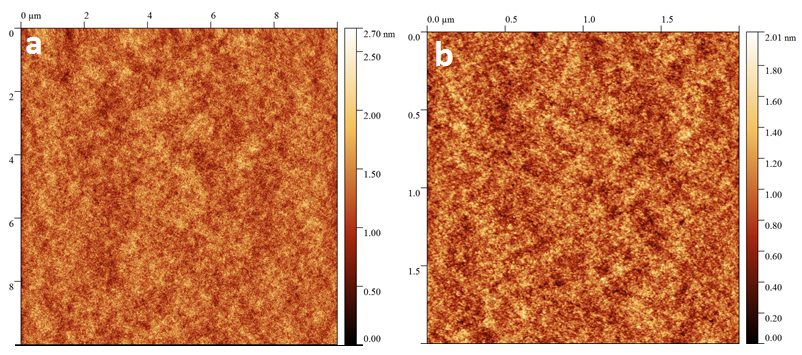
\includegraphics[width=120mm]{chapter3/Figure9.png}
\end{center}
\caption{Two sample AFM images of untreated borosilicate glass at two different scan sizes: (a) displays an image with a scan size of 10$\mu$m x 10$\mu$m, while (b) demonstrates a scan size of 2μm x 2μm.}
\label{fig:figure9}                 % Reference label to the figure.
\end{figure}   
  
The images produced showed a uniform surface across the 24 image dataset, with a maximum peak to peak roughness of 3.64nm for 10μm x 10μm images and 2.55nm for 2μm x 2μm images. Figure \ref{fig:figure9} demonstrates an example of each image per scan size, giving the general topology of the observed glass.
The observed images demonstrated that the topology and roughness of the capillary was constant across the entire length of the inside capillary as well as uniform across multiple capillaries. As a result of these images the capillaries used in the main investigation are assumed to demonstrate similar surface structure to figure \ref{fig:figure9}.

In order to ensure that any error incurred by physical error was accounted for an investigation into the x, y and z error was carried out. The AFM was left to image the same glass sample repeatedly in order to produce the same image several times. This image was then two dimensionally cross correlated with the next image in the sequence and the difference removed between the two z data points. The results are displayed in Figure\ref{fig:CrossCor}.

\begin{figure}[h]     %Insert a figure as soon as possible
        \begin{center}
          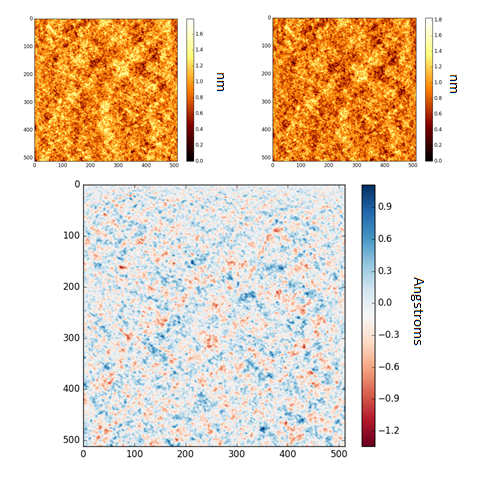
\includegraphics[width=120mm]{chapter3/CrossCor.png}
\end{center}
\caption{The output image of the 2D cross correlation function between the two images. The two smaller images are the input images into the script. The x and y values are the location of the z values in the 2D matrix dataset. The z scale is labeled respectively.}
\label{fig:CrossCor}                 % Reference label to the figure.
\end{figure}

Due to the drift experienced while scanning, the rows were found to be increasingly misaligned towards the bottom of the image.The result of this is shown by the gradient seen from the top of the image downwards , as the first image scanned from the bottom up, then the second image was scanned from the top down. The process was repeated on a row by row alignment basis and the resultant drift between the two images was found to be approximately 1 angstrom on the z axis, 8nm on the y axis and 28 on the x axis. However given the speed of the scan was low at 0.4Hz each image took approximately 40 minutes to image, giving an approximate drift of 0.1nm by 0.5nm drift per minute.

%SILICA TIP SURFACE

\section{Silica particle surface resolution} % MOVE TO CHAPTER 3 PLEASE

Successful resolution of a 1.5$\mu$m silica sphere was imaged under AFM and spherical deconvolution was processed with gwyddion. \cite{gwy} Futher work will be done to investigate adhesive forces between silica particles and to determine if the "pit" present in the center of the image is due to sonication.

\begin{figure}[h]     %Insert a figure as soon as possible
        \begin{center}
          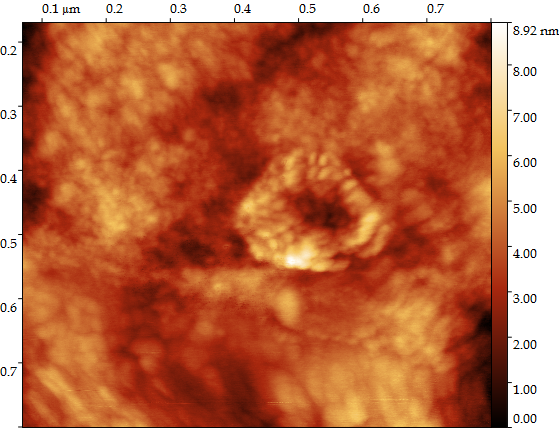
\includegraphics[width=130mm]{chapter4/Sili2.png}
\end{center}
\caption{The flattened surface of a silica sphere.}
\label{fig:Sili2}                 % Reference label to the figure.
\end{figure}


From the region any tilt or shift in the constant phase is taken away from the whole dataset. %What am I talk- oh, AFM image interpretation

\newpage
\newpage
\newpage

\section{Root mean squared roughness}
\newpage